\documentclass[12pt,a4paper]{article}

\usepackage{fontspec}
\IfFontExistsTF{Times New Roman}{\setmainfont{Times New Roman}}{%
  \IfFontExistsTF{Arial}{\setmainfont{Arial}}{\setmainfont{TeX Gyre Termes}}%
}
\usepackage{amsmath,amssymb}
\usepackage{unicode-math}
\IfFontExistsTF{Cambria Math}{\setmathfont{Cambria Math}}{}
\usepackage{geometry}
\geometry{top=1.25cm,bottom=1.15cm,left=1.50cm,right=1.50cm}
\usepackage{xcolor}
\usepackage{array}
\usepackage{booktabs}
\usepackage{float}
\usepackage{caption}
\usepackage{enumitem}
\captionsetup{skip=2pt,font=small,labelfont=bf}
\usepackage{fancyhdr}
\usepackage{tikz}
\usetikzlibrary{arrows.meta}
\usepackage{hyperref}
\hypersetup{colorlinks=true,linkcolor=blue!55!black,urlcolor=blue!55!black}

\setlength{\parindent}{0pt}
\setlength{\parskip}{2pt}
\setlength{\abovedisplayskip}{2pt}
\setlength{\belowdisplayskip}{2pt}
\renewcommand{\arraystretch}{1.05}
\renewcommand{\figurename}{Hình}
\renewcommand{\tablename}{Bảng}

\definecolor{criticalbar}{RGB}{211,47,47}
\definecolor{normalbar}{RGB}{63,125,190}

\pagestyle{fancy}
\fancyhf{}
\lhead{\small Quản trị dự án -- Bài 3}
\rhead{\small Bach Minh Quang -- 202490077}
\cfoot{\thepage}
\setlength{\headheight}{14pt}

\tikzset{
  event/.style={circle,draw=black,thick,minimum size=11.0mm,inner sep=0.2pt,
    font=\scriptsize\bfseries,align=center,fill=white},
  arc/.style={-{Latex[length=2.1mm]},thick,normalbar},
  criticalarc/.style={-{Latex[length=2.1mm]},very thick,criticalbar},
  dummyarc/.style={-{Latex[length=2.1mm]},dashed,thick,gray!65!black},
  arclabel/.style={font=\scriptsize\bfseries,fill=white,inner sep=1pt}
}

\begin{document}

\begin{center}
  {\large\bfseries ĐẠI HỌC BÁCH KHOA HÀ NỘI}\\[0.4pt]
  {\bfseries Trường Công nghệ Thông tin và Truyền thông}\\[3.5pt]
  {\Large\bfseries BÀI TẬP 3 -- SƠ ĐỒ PERT}\\[0.5pt]
  {\small Bach Minh Quang \quad MSSV: 202490077 \quad Hà Nội, 09/2026}
\end{center}
\vspace{-2pt}
\hrule
\vspace{5pt}

\paragraph{Dữ liệu.}
Vẽ sơ đồ PERT, tính các yếu tố thời gian, các loại dự trữ và xác định đường găng.
Số liệu công việc như sau.

\begin{table}[H]\centering
\caption{Dữ liệu công việc -- Bài 3}
\small
\begin{tabular}{cccccc}
\toprule
\textbf{CV} & \textbf{Trình tự} & \textbf{$d$} &
\textbf{CV} & \textbf{Trình tự} & \textbf{$d$}\\
\midrule
$A$ & Từ đầu & 3 & $I$ & Sau $C$ & 6\\
$B$ & Từ đầu & 4 & $K$ & Sau $F$ & 3\\
$C$ & Từ đầu & 4 & $L$ & Sau $F$ & 10\\
$D$ & Sau $A$ & 5 & $M$ & Sau $F$, $I$ & 9\\
$G$ & Sau $D$ & 5 & $N$ & Sau $H$, $K$ & 7\\
$H$ & Sau $A$ & 9 & $P$ & Sau $L$, $M$, $N$ & 12\\
$F$ & Sau $B$, $G$ & 7 & & & \\
\bottomrule
\end{tabular}
\end{table}

\paragraph{a. Sơ đồ PERT.}
Mạng AOA. Mũi đỏ: công việc găng. Mũi xanh: không găng. Nét đứt: việc giả ($d=0$).
Trong đỉnh: số hiệu sự kiện và $t_s/t_m$.
Năm việc giả:
$e_1$ nối kết thúc $B$ vào đầu $F$;
$e_2$ nối kết thúc $F$ vào đầu $M$;
$e_3$ nối kết thúc $I$ vào đầu $M$;
$e_4$ nối kết thúc $H$ vào đầu $N$;
$e_5$ nối kết thúc $M$ vào đầu $P$.

\begin{figure}[H]\centering
\resizebox{0.99\linewidth}{!}{%
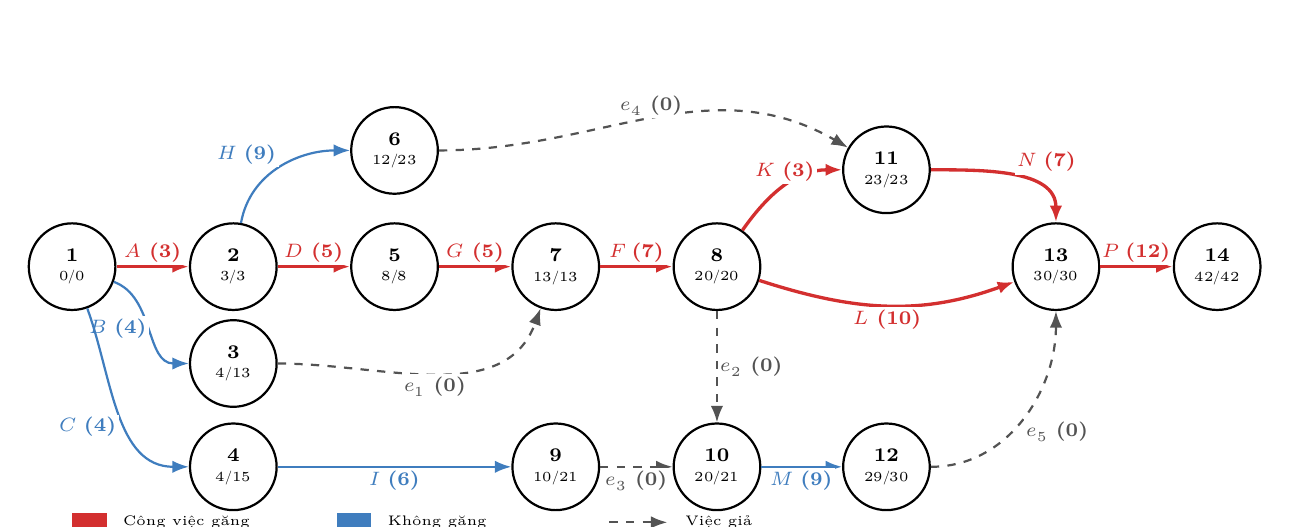
\begin{tikzpicture}[x=1.05cm,y=0.82cm]
  \node[event] (p1)  at (0.00,1.55) {1\\[-1pt]{\tiny\normalfont $0/0$}};
  \node[event] (p2)  at (1.95,1.55) {2\\[-1pt]{\tiny\normalfont $3/3$}};
  \node[event] (p3)  at (1.95,0.05) {3\\[-1pt]{\tiny\normalfont $4/13$}};
  \node[event] (p4)  at (1.95,-1.55) {4\\[-1pt]{\tiny\normalfont $4/15$}};
  \node[event] (p6)  at (3.90,3.35) {6\\[-1pt]{\tiny\normalfont $12/23$}};
  \node[event] (p5)  at (3.90,1.55) {5\\[-1pt]{\tiny\normalfont $8/8$}};
  \node[event] (p7)  at (5.85,1.55) {7\\[-1pt]{\tiny\normalfont $13/13$}};
  \node[event] (p9)  at (5.85,-1.55) {9\\[-1pt]{\tiny\normalfont $10/21$}};
  \node[event] (p8)  at (7.80,1.55) {8\\[-1pt]{\tiny\normalfont $20/20$}};
  \node[event] (p10) at (7.80,-1.55) {10\\[-1pt]{\tiny\normalfont $20/21$}};
  \node[event] (p11) at (9.85,3.05) {11\\[-1pt]{\tiny\normalfont $23/23$}};
  \node[event] (p12) at (9.85,-1.55) {12\\[-1pt]{\tiny\normalfont $29/30$}};
  \node[event] (p13) at (11.90,1.55) {13\\[-1pt]{\tiny\normalfont $30/30$}};
  \node[event] (p14) at (13.85,1.55) {14\\[-1pt]{\tiny\normalfont $42/42$}};

  \draw[criticalarc] (p1) -- node[arclabel,above] {$A$ (3)} (p2);
  \draw[arc] (p1) to[out=-20,in=180] node[arclabel,left] {$B$ (4)} (p3);
  \draw[arc] (p1) to[out=-70,in=180] node[arclabel,below left] {$C$ (4)} (p4);
  \draw[criticalarc] (p2) -- node[arclabel,above] {$D$ (5)} (p5);
  \draw[arc] (p2) to[out=80,in=180] node[arclabel,above left] {$H$ (9)} (p6);
  \draw[criticalarc] (p5) -- node[arclabel,above] {$G$ (5)} (p7);
  \draw[dummyarc] (p3) to[out=0,in=-110] node[arclabel,below] {$e_1$ (0)} (p7);
  \draw[criticalarc] (p7) -- node[arclabel,above] {$F$ (7)} (p8);
  \draw[arc] (p4) -- node[arclabel,below] {$I$ (6)} (p9);
  \draw[criticalarc] (p8) to[out=55,in=180] node[arclabel,above] {$K$ (3)} (p11);
  \draw[criticalarc] (p8) to[out=-18,in=200] node[arclabel,below] {$L$ (10)} (p13);
  \draw[dummyarc] (p8) -- node[arclabel,right] {$e_2$ (0)} (p10);
  \draw[dummyarc] (p9) -- node[arclabel,below] {$e_3$ (0)} (p10);
  \draw[arc] (p10) -- node[arclabel,below] {$M$ (9)} (p12);
  \draw[dummyarc] (p6) to[out=0,in=150] node[arclabel,above] {$e_4$ (0)} (p11);
  \draw[criticalarc] (p11) to[out=0,in=90] node[arclabel,above right] {$N$ (7)} (p13);
  \draw[dummyarc] (p12) to[out=0,in=-90] node[arclabel,below right] {$e_5$ (0)} (p13);
  \draw[criticalarc] (p13) -- node[arclabel,above] {$P$ (12)} (p14);

  \fill[criticalbar] (0.00,-2.55) rectangle +(0.42,0.28);
  \node[anchor=west,font=\tiny] at (0.50,-2.41) {Công việc găng};
  \fill[normalbar] (3.20,-2.55) rectangle +(0.42,0.28);
  \node[anchor=west,font=\tiny] at (3.70,-2.41) {Không găng};
  \draw[dummyarc] (6.50,-2.41) -- +(0.70,0);
  \node[anchor=west,font=\tiny] at (7.30,-2.41) {Việc giả};
\end{tikzpicture}}
\caption{Mạng PERT. Hai đường găng $A$--$D$--$G$--$F$--$L$--$P$ và $A$--$D$--$G$--$F$--$K$--$N$--$P$.}
\end{figure}

\paragraph{b. Chỉ tiêu các sự kiện.}
Tính tiến: $t_s(j)=\max_{i\rightarrow j}\{t_s(i)+d_{ij}\}$, $t_s(1)=0$.
Tính lùi: $t_m(i)=\min_{i\rightarrow j}\{t_m(j)-d_{ij}\}$, $t_m(14)=t_s(14)$.
Dự trữ đỉnh $R(i)=t_m(i)-t_s(i)$; đỉnh găng khi $R=0$.

{\footnotesize
\begin{minipage}[t]{0.49\textwidth}
\textbf{Tiến}\\[1pt]
$t_s(1)=0$\\
$t_s(2)=0+3=3$\\
$t_s(3)=0+4=4$\\
$t_s(4)=0+4=4$\\
$t_s(5)=3+5=8$\\
$t_s(6)=3+9=12$\\
$t_s(7)=\max\{8+5,\ 4+0\}=13$\\
$t_s(8)=13+7=20$\\
$t_s(9)=4+6=10$\\
$t_s(10)=\max\{20+0,\ 10+0\}=20$\\
$t_s(11)=\max\{20+3,\ 12+0\}=23$\\
$t_s(12)=20+9=29$\\
$t_s(13)=\max\{20+10,\ 23+7,\ 29+0\}=30$\\
$t_s(14)=30+12=42$
\end{minipage}
\hfill
\begin{minipage}[t]{0.49\textwidth}
\textbf{Lùi}\\[1pt]
$t_m(14)=42$\\
$t_m(13)=42-12=30$\\
$t_m(12)=30-0=30$\\
$t_m(11)=30-7=23$\\
$t_m(10)=30-9=21$\\
$t_m(9)=21-0=21$\\
$t_m(8)=\min\{23-3,\ 30-10,\ 21-0\}=20$\\
$t_m(7)=20-7=13$\\
$t_m(6)=23-0=23$\\
$t_m(5)=13-5=8$\\
$t_m(4)=21-6=15$\\
$t_m(3)=13-0=13$\\
$t_m(2)=\min\{8-5,\ 23-9\}=3$\\
$t_m(1)=\min\{3-3,\ 13-4,\ 15-4\}=0$
\end{minipage}
}

\begin{table}[H]\centering
\caption{Thời điểm sớm, muộn và dự trữ các sự kiện}
\scriptsize
\begin{tabular}{c|rrrrrrrrrrrrrr}
\toprule
Sự kiện $i$ & 1 & 2 & 3 & 4 & 5 & 6 & 7 & 8 & 9 & 10 & 11 & 12 & 13 & 14\\
\midrule
$t_s(i)$ & 0 & 3 & 4 & 4 & 8 & 12 & 13 & 20 & 10 & 20 & 23 & 29 & 30 & 42\\
$t_m(i)$ & 0 & 3 & 13 & 15 & 8 & 23 & 13 & 20 & 21 & 21 & 23 & 30 & 30 & 42\\
$R(i)$   & 0 & 0 & 9 & 11 & 0 & 11 & 0 & 0 & 11 & 1 & 0 & 1 & 0 & 0\\
\bottomrule
\end{tabular}
\end{table}

Đỉnh găng: $1,2,5,7,8,11,13,14$.
Thời gian sớm nhất hoàn thành dự án: $T=t_s(14)=t_m(14)=\mathbf{42}$ ngày.

\paragraph{Các yếu tố thời gian của công việc.}
Với cung $i\rightarrow j$:
$ES=t_s(i)$, $EF=t_s(i)+d$, $LS=t_m(j)-d$, $LF=t_m(j)$,
$TF=t_m(j)-t_s(i)-d$,
$FF=t_s(j)-t_s(i)-d$,
$IF=\max\{0,\ t_s(j)-t_m(i)-d\}$.

\begin{table}[H]\centering
\caption{Chỉ tiêu thời gian các công việc}
\small
\begin{tabular}{c|c|c|rr|rr|rrr}
\toprule
\textbf{CV} & $i\!\rightarrow\!j$ & $d$ & ES & EF & LS & LF & TF & FF & IF\\
\midrule
$A$ & $1\rightarrow 2$ & 3 & 0 & 3 & 0 & 3 & \textbf{0} & 0 & 0\\
$B$ & $1\rightarrow 3$ & 4 & 0 & 4 & 9 & 13 & 9 & 0 & 0\\
$C$ & $1\rightarrow 4$ & 4 & 0 & 4 & 11 & 15 & 11 & 0 & 0\\
$D$ & $2\rightarrow 5$ & 5 & 3 & 8 & 3 & 8 & \textbf{0} & 0 & 0\\
$G$ & $5\rightarrow 7$ & 5 & 8 & 13 & 8 & 13 & \textbf{0} & 0 & 0\\
$H$ & $2\rightarrow 6$ & 9 & 3 & 12 & 14 & 23 & 11 & 0 & 0\\
$F$ & $7\rightarrow 8$ & 7 & 13 & 20 & 13 & 20 & \textbf{0} & 0 & 0\\
$I$ & $4\rightarrow 9$ & 6 & 4 & 10 & 15 & 21 & 11 & 0 & 0\\
$K$ & $8\rightarrow 11$ & 3 & 20 & 23 & 20 & 23 & \textbf{0} & 0 & 0\\
$L$ & $8\rightarrow 13$ & 10 & 20 & 30 & 20 & 30 & \textbf{0} & 0 & 0\\
$M$ & $10\rightarrow 12$ & 9 & 20 & 29 & 21 & 30 & 1 & 0 & 0\\
$N$ & $11\rightarrow 13$ & 7 & 23 & 30 & 23 & 30 & \textbf{0} & 0 & 0\\
$P$ & $13\rightarrow 14$ & 12 & 30 & 42 & 30 & 42 & \textbf{0} & 0 & 0\\
\bottomrule
\end{tabular}
\end{table}

\paragraph{Đường găng.}
\enlargethispage{3\baselineskip}
Công việc găng khi $TF=0$: $A,D,G,F,K,L,N,P$.
Đối chiếu các đường đi từ 1 đến 14:
\begin{itemize}[leftmargin=1.4em,itemsep=1pt,parsep=0pt,topsep=2pt]
  \item $A$--$D$--$G$--$F$--$L$--$P$: $3+5+5+7+10+12=\mathbf{42}$
  \item $A$--$D$--$G$--$F$--$K$--$N$--$P$: $3+5+5+7+3+7+12=\mathbf{42}$
  \item $A$--$D$--$G$--$F$--$e_2$--$M$--$e_5$--$P$: $3+5+5+7+0+9+0+12=41$
  \item $A$--$H$--$e_4$--$N$--$P$: $3+9+0+7+12=31$
  \item $B$--$e_1$--$F$--$L$--$P$: $4+0+7+10+12=33$
  \item $C$--$I$--$e_3$--$M$--$e_5$--$P$: $4+6+0+9+0+12=31$
\end{itemize}
\vspace{-4pt}
\[
  \boxed{A\text{--}D\text{--}G\text{--}F\text{--}L\text{--}P
  \quad\text{và}\quad
  A\text{--}D\text{--}G\text{--}F\text{--}K\text{--}N\text{--}P
  \qquad (42\ \text{ngày})}
\]
\vspace{-6pt}
{\small
Công việc không găng: $B$ ($TF=9$), $C$, $H$, $I$ ($TF=11$), $M$ ($TF=1$).
Mọi $IF=0$. Kéo dài đồng thời bị chặn bởi $M$ (đường 41 ngày), mức chung lớn nhất là \textbf{1 ngày}.}

\end{document}
